   
        \section{Overview of multivariate functions}
        Aside from the study of linear transformations on $\R^n$ or $\C^n$, we have limited ourselves to functions of a single variable.  Given that we have performed a deep analysis for functions of one variable, we can take what we have learned and apply it to new types of functions. Specifically, we will concentrate on $\R^3$ (or $\R^2$) and functions of the form:
        \begin{align*}
            &\curvegamma\colon \R \to \R^3\\
            &f\colon \R^3 \to \R\\
            &\forcevec \colon \R^3 \to \R^3.
        \end{align*}
        Of these three functions, the latter two are often referred to as \boldgreen{fields}.  These are also \boldgreen{multivariate} functions, whereas the first only has an input of a single variable.
        
        
        \begin{enumerate}[(1)]
        \item Functions of the form
        \[
        \curvegamma \colon \R\to \R^3
        \]
        are \boldgreen{curves}.  Often times, we will have 
        \[
        \curvegamma \colon [a,b]\to \R^3
        \]
        when we want curves with specific endpoints. We will concentrate first on curves, so I'll save the extra detail for a bit later.
        
        \item Functions of the form
        \[
        f\colon \R^3 \to \R
        \]
        are \boldgreen{scalar fields} .   These functions are useful in describing quantities like temperature in space.  In this example, at each point $\vecx$ in space $\R^3$, we can assign a single real number output $f(\vecx)$ that tells us this temperature.  
        
        %One may ask how this function changes from point to point.  Asking this question sends you immediately to investigating the \emph{gradient}.  It turns out, using our temperature example, that we can understand heat flow by understanding temperature gradients.
        
        \item Functions of the form
        \[
        \forcevec\colon \R^3 \to \R^3
        \]
        are called \boldgreen{vector fields}.  Roughly speaking, at each point $\vecx$ in space $\R^3$, we can place a vector $\forcevec(\vecx)$ that is also in $\R^3$.  These fields are very important in describing systems that have flow.  For example, fluid flow or electromagnetism are vector field theories. 
        
        % What will it mean to find the change in a vector field?  This will lead us to the notion of the \emph{total derivative}.  This concept is a bit abstract at first but will really tell us the proper notion of the derivative.
        \end{enumerate}
        
        
        \section{Curves in space}
        
        We will begin with curves as they are very useful tools and this will help us visualize results for the other types of functions. 
        
        Let us consider a curve
        \[
        \curvegamma \colon \R \to \R^3.
        \]
        We will specify a specific curve by supplying three functions $f_1(t)$, $f_2(t)$, and $f_3(t)$. Specifically, each of these functions $f_i$ is a function $f_i\colon \R \to \R$. Then, we can say that
        \[
        \gamma(t)=(f_1(t),f_2(t),f_3(t))=\begin{bmatrix} f_1(t)\\ f_2(t)\\ f_3(t)\end{bmatrix}.
        \]
        \emph{Note, I will likely use these above notations for vectors interchangeably.} 
        
        Each $f_i(t)$ (for the values $i=1,2,3$) is called a \textbf{coordinate function}.  Intuitively, the coordinate function tells us where the curve is at a time $t$. That is
        \begin{align*}
            &f_1(t) \quad \textrm{the $x$-position of $\gamma$ at time $t$,}\\
            &f_2(t) \quad \textrm{the $y$-position of $\gamma$ at time $t$,}\\
            &f_3(t) \quad \textrm{the $z$-position of $\gamma$ at time $t$.}
        \end{align*}
        The nice thing about these coordinate functions is we entirely know how to deal with their calculus since each is a function $f_i\colon \R \to \R$.
        
        Now, we can find the \textbf{tangent vector} or \textbf{velocity vector} to the curve $\gamma$ at a time $t$.  We covered this in the complex case, and the idea here is arguably more straightforward. 
        
        Imagine that $\gamma(t)$ is the position of a small particle at the time $t$.  Then the velocity is the time rate of change of this position.  Specifically, we see how each of the coordinate functions changes, and this will tell us how the position changes! So, we have the following.
        
        \begin{df}{Tangent Vector to a Curve}{tang_to_curve}
        Given a curve $\gamma$, the \textbf{tangent vector to $\gamma$ at the time $t$} is
        \[
        \gamma'(t)=\lim_{\delta \to 0} \frac{\gamma(t+\delta)-\gamma(t)}{\delta}.
        \]
        It turns out that we find $\gamma'$ is
        \[
        \gamma'(t)=(f_1'(t),f_2'(t),f_3'(t))=\begin{bmatrix} f_1'(t)\\ f_2'(t)\\ f_3'(t)\end{bmatrix}.
        \]
        \end{df}
        
        \begin{ex}{Graph of a Quadratic Function}{graph_quad}
        Consider the curve $\gamma\colon \R \to \R^2$ given by
        \[
        \gamma(t)=(t,t^2).
        \]
        This curve looks exactly like the graph of the function $f(x)=x^2$ that we have drawn many times before. 
        \begin{figure}[H]
            \centering
            \includegraphics[width=.4\textwidth]{Figures_Part_6/quadratic_curve.png}
        \end{figure}
        
        What is the tangent vector at time $t$? We have
        \[
        \gamma'(t)=(1,2t).
        \]
        If we take this $y$-value over the $x$-value we arrive at the same conclusion for the derivative to $f(x)=x^2$ (i.e., $f'(x)=2x$).
        \end{ex}
        
        \begin{ex}{Circle Curve}{circ_curve}
        Consider the curve $\gamma \colon [0,1] \to \R^2$ given by
        \[
        \gamma(t)=(\cos (2\pi t),\sin (2\pi t)).
        \]
        This curve is a circle of radius $1$ centered at $(0,0)$.  We can find the tangent vector at a time $t$ by
        \[
        \gamma'(t)=(-2\pi \sin(2\pi t), 2\pi \cos(2\pi t)).
        \]
        See the following graphs
        
    \begin{figure}[H]
    \centering
    \begin{subfigure}[h]{0.45\textwidth}
        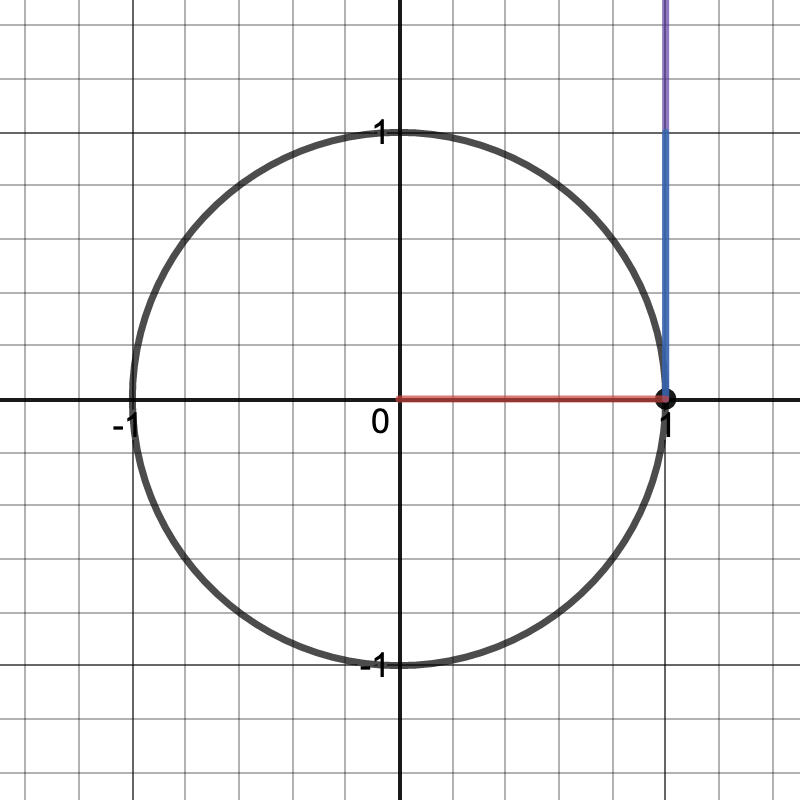
\includegraphics[width=\textwidth]{Figures_Part_6/circ_tang_1.png}
        \caption{Tangent vector at $t=0$.}
    \end{subfigure}
    ~ 
    \begin{subfigure}[h]{0.45\textwidth}
        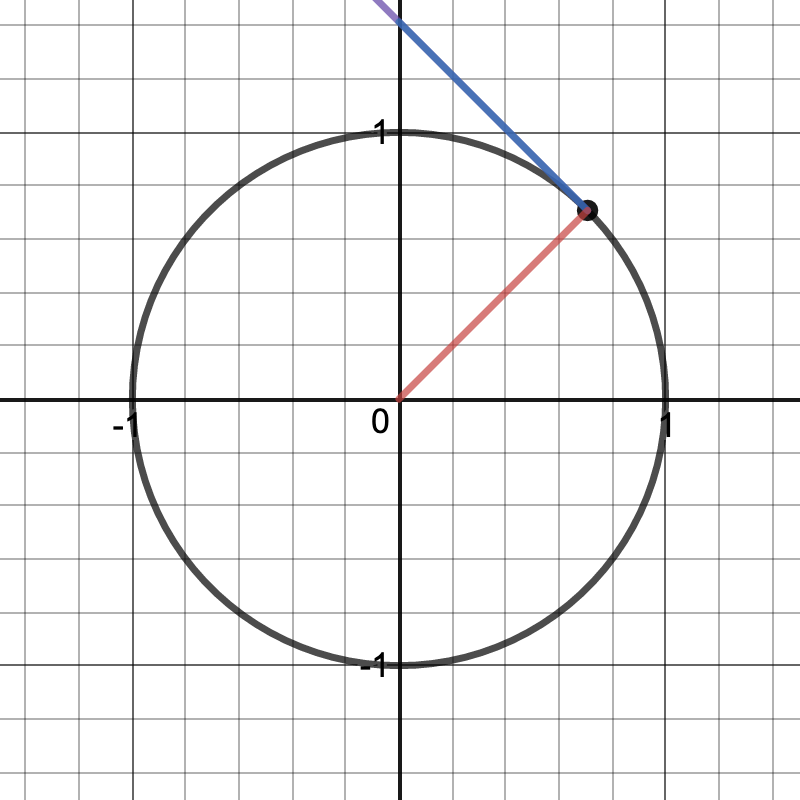
\includegraphics[width=\textwidth]{Figures_Part_6/circ_tang_2.png}
        \caption{Tangent vector at $t=\frac{1}{8}$.}
    \end{subfigure}
    
    \begin{subfigure}[h]{0.45\textwidth}
        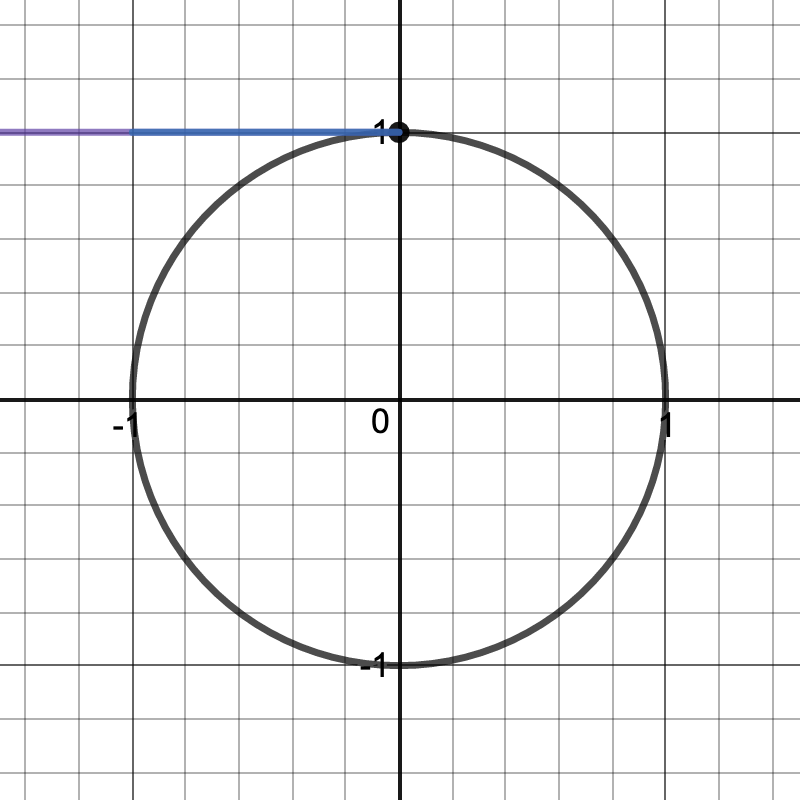
\includegraphics[width=\textwidth]{Figures_Part_6/circ_tang_3.png}
        \caption{Tangent vector at $t=\frac{1}{4}$.}
    \end{subfigure}
    ~
    \begin{subfigure}[h]{0.45\textwidth}
        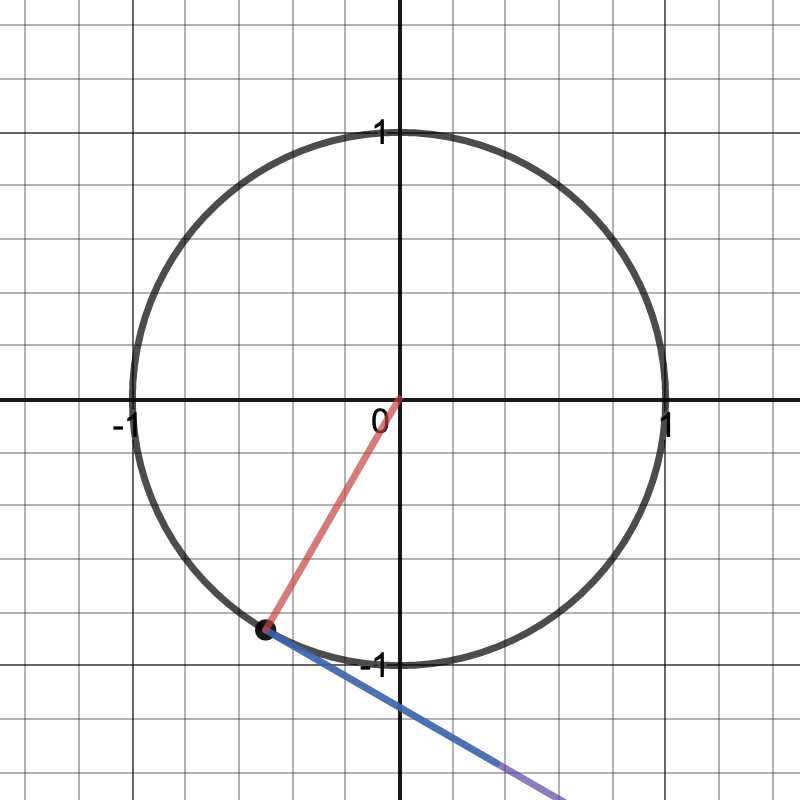
\includegraphics[width=\textwidth]{Figures_Part_6/circ_tang_4.png}
        \caption{Tangent vector at $t=\frac{2}{3}$.}
    \end{subfigure}
        \end{figure}
        
        We can also compute the \textbf{normal vector} or \textbf{acceleration vector} to a curve by taking another derivative.  We write
        \[
        \gamma''(t)=(-4\pi^2 \cos(2\pi t),-4\pi^2 \sin(2\pi t)).
        \]
        \end{ex}
        
        \subsubsection{Line integrals}
        
        In reality, we like to add up function values along curves.  We have already done this before in the complex case with contours.  You also did this in a calculus I course via the Riemann integral.  We will get to this, but we need to know the correct functions to add up along a curve first. These will be the vector and scalar fields fields.
        
        
%        
%        \section{Scalar fields}
%        The next major class of functions we will consider are the scalar fields.  That is, functions that take the form
%        \[
%        f\colon \R^3 \to \R.
%        \]
%        Often, it will be helpful to visualize functions by considering instead
%        \[
%        f\colon \R^2 \to \R
%        \]
%        and looking at the \emph{graph} of $f$.  
%        
%        \begin{ex}{Graph of a function}{graph_of_func}
%        Whenever we talk of a function of the form
%        \[
%        f\colon \R \to \R
%        \]
%        we inherently tend to draw the graph of the function $f$.  By graph, I mean that given $f$, we usually just draw $(x,f(x))$ in the plane.
%        
%        Take for example, $f\colon \R \to \R$ given by $f(x)=x^2$.  We usually draw the plane $\R^2$ and graph the curve $(x,f(x))$ which looks like
%        \begin{figure}[H]
%            \centering
%            \includegraphics[width=.5\textwidth]{Figures/quadratic_curve.png}           
%        \end{figure}
%        All of this is to say that graphs of these types of functions are special kinds of curves.  In other words, they are curves that pass the vertical line test.
%        \end{ex}
%        
%        \begin{ex}{The Paraboloid}{paraboloid}
%        Let $f\colon \R^2 \to \R$ be given by
%        \[
%        f(x,y)=x^2+y^2.
%        \]
%        We can plot the graph of the function by plotting $(x,y, f(x,y))$ in $\R^3$.  This will look like:
%        \begin{figure}[H]
%            \centering
%            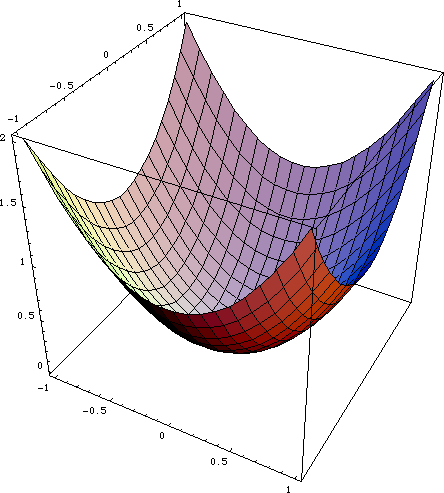
\includegraphics[width=.4\textwidth]{Figures/paraboloid.png}
%        \end{figure}
%        Then we can analyze this function in a few nice ways.  
%        
%        If we fix a value for $x$ or $y$, then we will be able to look at $f$ as a function of just a single variable.  
%        \begin{itemize}
%        \item So we can, for example, fix $y=0$ and then we have
%        \[
%        f(x,0)=x^2.
%        \]
%        So along the $y=0$ line, the function is just the parabola we are used to! 
%        
%        \item Similarly, we can force $x=0$ and arrive at
%        \[
%        f(0,y)=y^2
%        \]
%        is also a parabola.  
%        
%        \item But we are not limited to these choices.  We could have chosen $y=5$ and we would have
%        \[
%        f(x,5)=x^2+25
%        \]
%        which is a parabola shifted upwards by 25 units.
%        
%        \item  Again, we could also choose yet another ``slice" of this function and let $x=y$ which would give us
%        \[
%        f(x,x)=x^2+x^2=2x^2.
%        \]
%        So, along the $x=y$ line, the parabola is scaled by 2.
%        
%        \item One other method of analyzing this function would be to find what the \textbf{level curves} of this function are.  What are the points $(x,y)$ that satisfy $f(x,y)=c$?  We call these level curves much in the way that a topographical map plots curves along the areas with equal height.  For this example, consider the set of points $(x,y)$ so that $f(x,y)=1.$ This means
%        \[
%        f(x,y)=1=x^2+y^2.
%        \]
%        Since we have
%        \[
%        x^2+y^2=1
%        \]
%        that means each level curve is a circle!
%        \item Here is a ``topographical map" for this function (i.e., a plot of the level curves for this paraboloid.)
%        \begin{figure}[H]
%            \centering
%            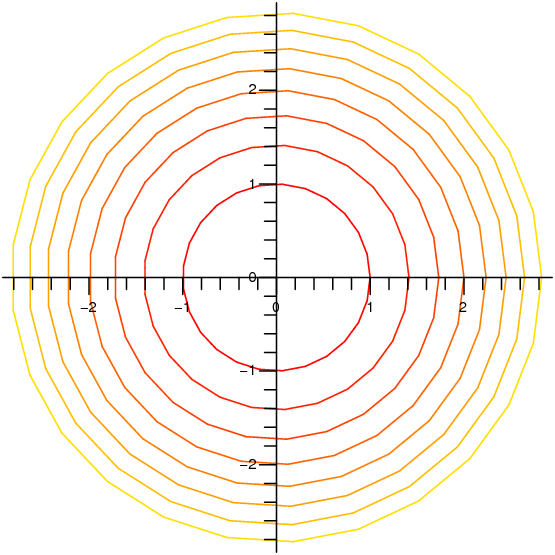
\includegraphics[width=.4\textwidth]{Figures/parabolic_level_curves.png}
%        \end{figure}
%        Here, each circle represents $f(x,y)=c$ for different values of $c$.  This really \emph{is} a topographical map!
%        \end{itemize}
%        \end{ex}
%        
%        \begin{exercise}[Plane]
%        Repeat this analysis for yourself for the following function:
%        \[
%        f(x,y)=x+y.
%        \]
%        \end{exercise}
%        
%        \section{Level surfaces}
%        In the planar case, we would often have to specify a set of points like
%        \[
%        x^2+y^2=1
%        \]
%        which is the circle.  
%        
%        In higher dimensions, we can do the same in order to visualize functions of the form $f\colon \R^3\to \R$ written as $f(x,y,z)$.  If we pick some constant $c$ and write
%        \[
%        f(x,y,z)=c
%        \]
%        then we will get the \textbf{level surfaces} for the function $f(x,y,z)$.  Visualizing functions of three variables (or more) $f(x,y,z)$ requires us to visualize in four or more dimensions. So we often reduce the problem to visualizing level surfaces.
%        
%        \begin{ex}{A Sphere as a Level Surface}{sphere_lev_surf}
%        We can consider the following function
%        \[
%        f(x,y,z)=x^2+y^2+z^2.
%        \]
%        If we take the one level set, that is the points $(x,y,z)$ that satisfy
%        \[
%        x^2+y^2+z^2=1
%        \]
%        then we get the \emph{2-sphere}.  These are the set of points that are all a distance one from the origin.  Here is a picture:
%        \begin{figure}[H]
%            \centering
%            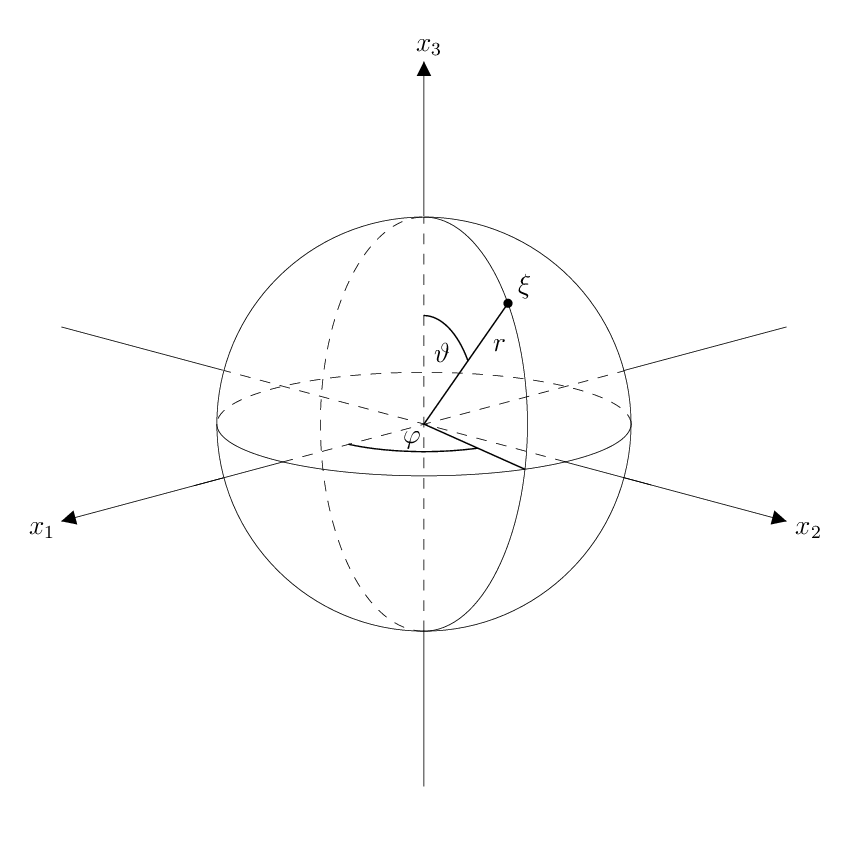
\includegraphics[width=.4\textwidth]{Figures/sphere.png}
%        \end{figure}
%        \end{ex}
%        
%        \begin{ex}{The Hyperboloids}{hyperboloids}
%        Consider a family of surfaces given by the level surfaces of
%        \[
%        f(x,y,z)=x^2+y^2-z^2.
%        \]
%        \begin{itemize}
%            \item If we take $c=0$ and set
%            \[
%            x^2+y^2-z^2=0.
%            \]
%            then we find the 0 level surface. In this case, we can do a bit of work to find
%            \[
%            z=\pm \sqrt{x^2+y^2}.
%            \]
%            Notice, if we pick any value for $z$, that we get a circle at that level!  When $z=0$, we get a single point.  It turns out that we get the \emph{(double) cone} surface which looks like
%            \begin{figure}[H]
%                \centering
%             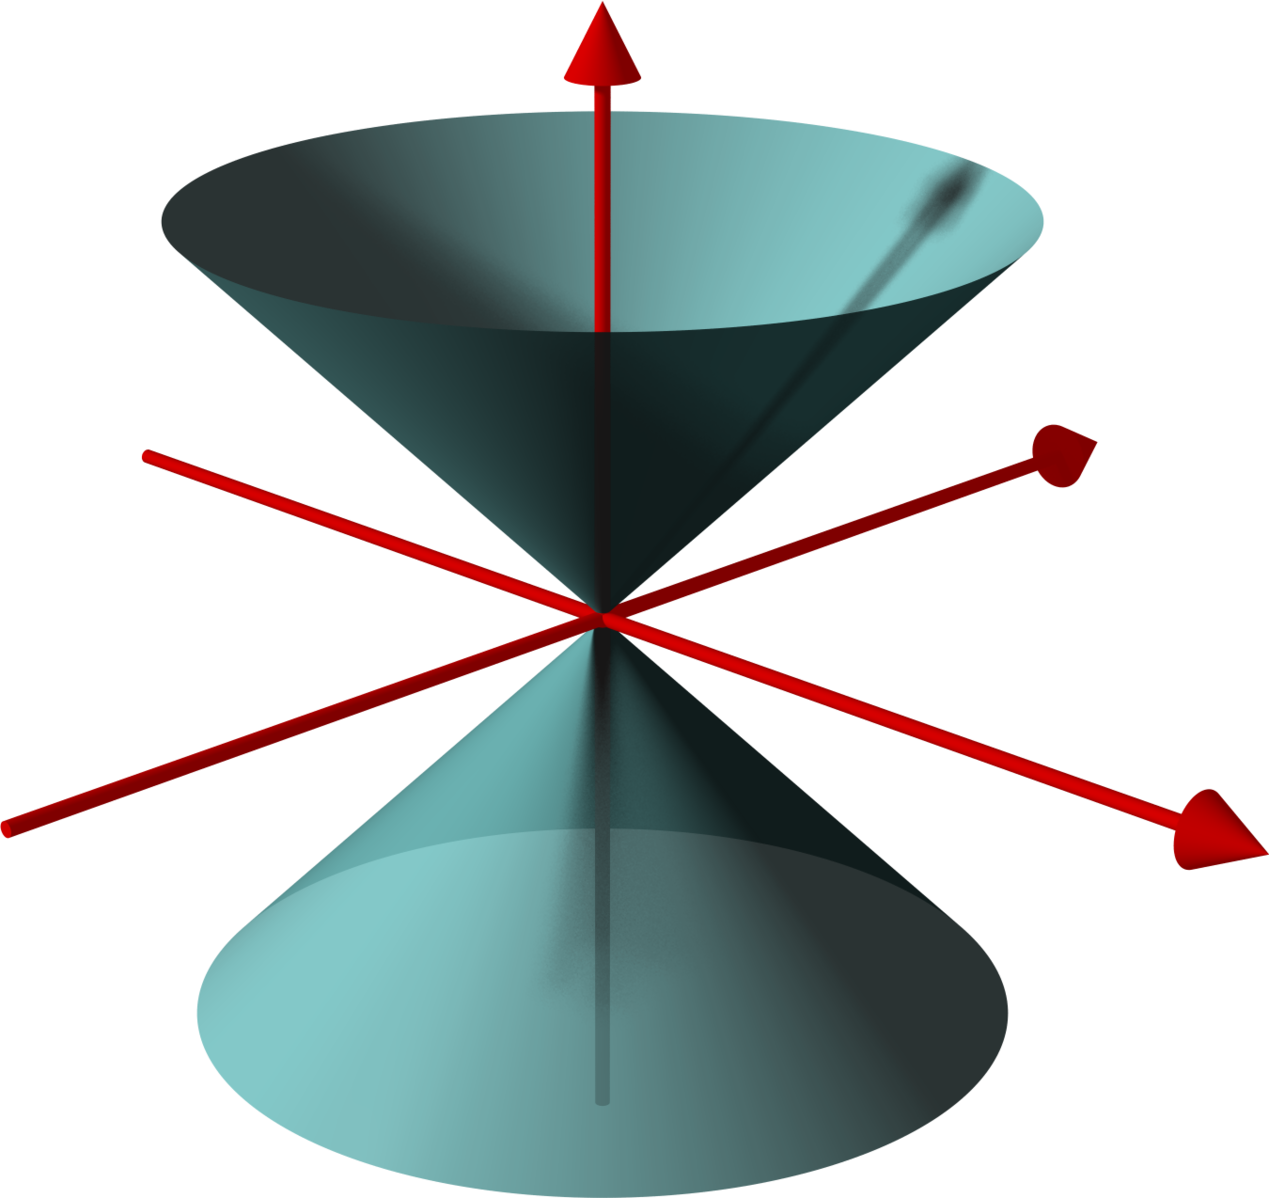
\includegraphics[width=.4\textwidth]{Figures/cone_surface.png}
%            \end{figure}
%            
%            \item If we take $c=1$ and set
%            \[
%            x^2+y^2-z^2=1
%            \]
%            we get the \emph{hyperboloid of one sheet}.  This looks like
%            \begin{figure}[H]
%                \centering
%                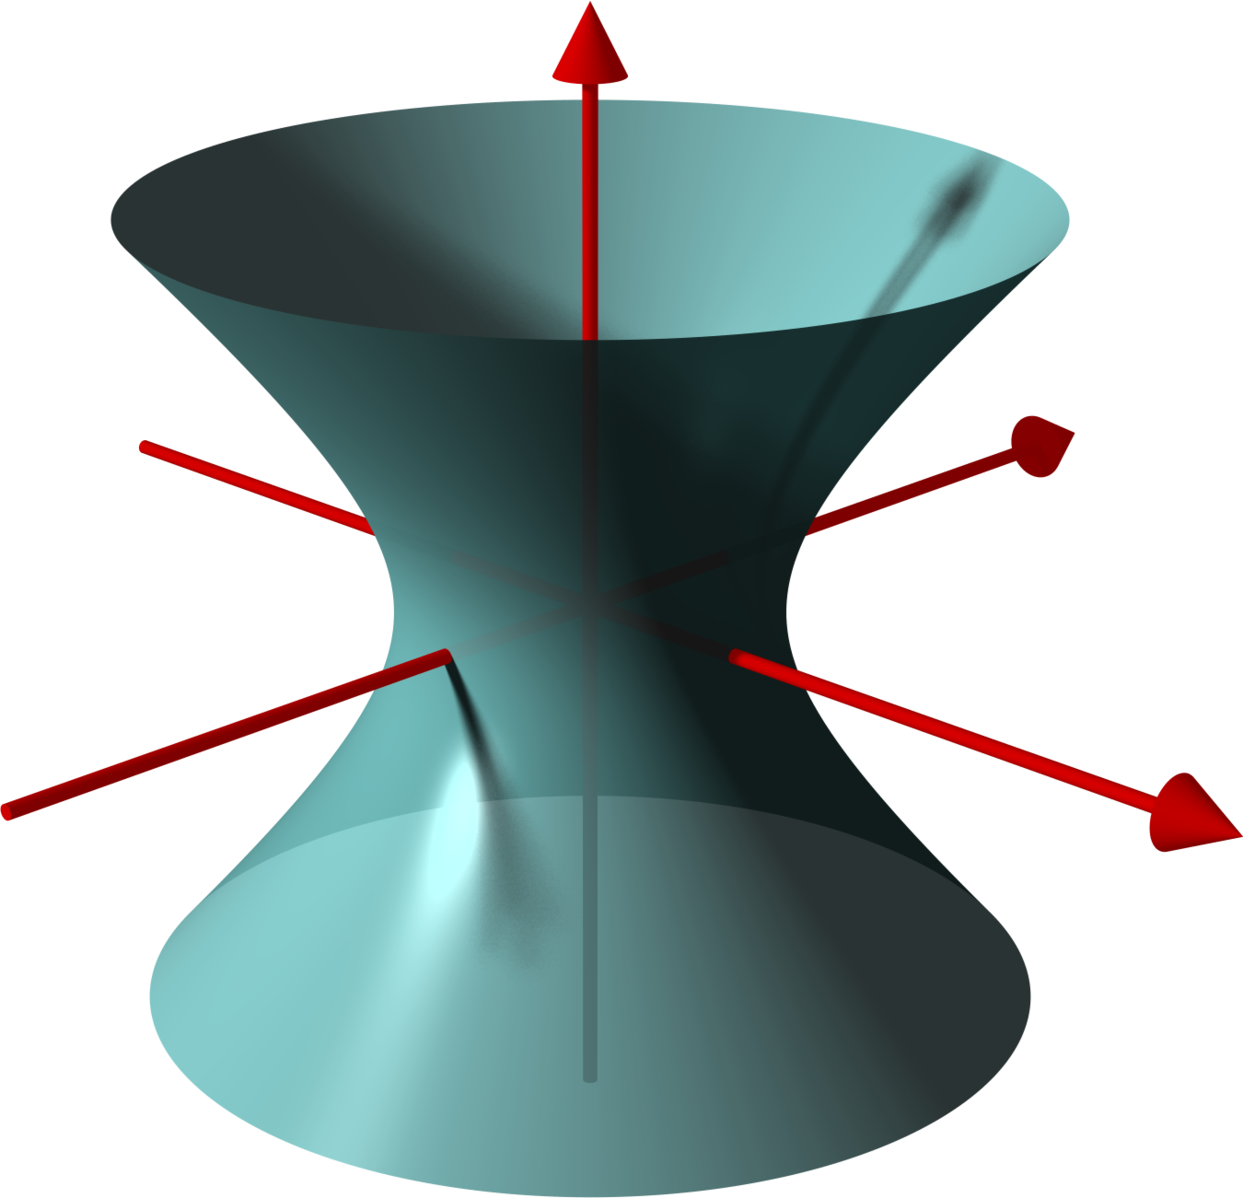
\includegraphics[width=.4\textwidth]{Figures/hyperboloid_1_sheet.png}
%            \end{figure}
%            
%            \item If we take $c=-1$ and set
%            \[
%            x^2+y^2-z^2=-1
%            \]
%            we get the \emph{hyperboloid of two sheets}.  This looks like
%            \begin{figure}[H]
%                \centering
%                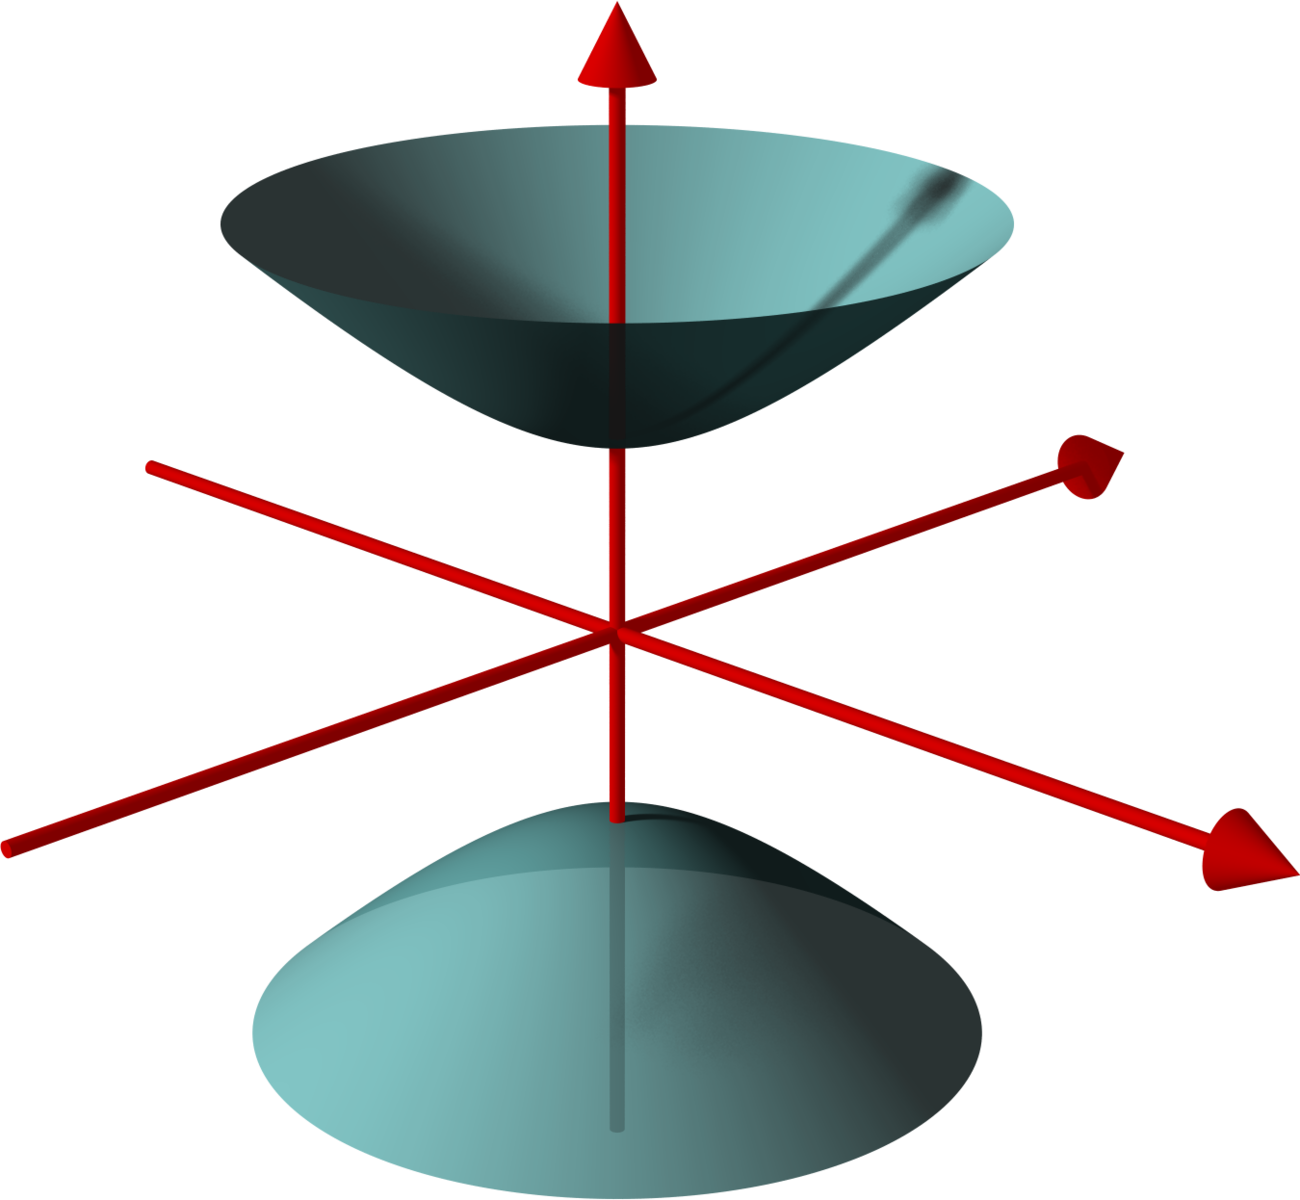
\includegraphics[width=.4\textwidth]{Figures/hyperboloid_2_sheet.png}
%            \end{figure}
%        \end{itemize}
%        \end{ex}
%        
%        \begin{ex}{The Torus}{torus}
%        For this example, I will choose specific nice numbers, but this is a yet another case of a level surface.  Take
%        \[
%        \left(5-\sqrt{x^2+y^2}\right)^2+z^2=2.
%        \]
%        This gives us the \emph{torus} with inner radius (the radius from the center of the donut hole to the center of the tube) $5=R$ and tube radius $2=r$. This looks like
%        \begin{figure}[H]
%            \centering
%            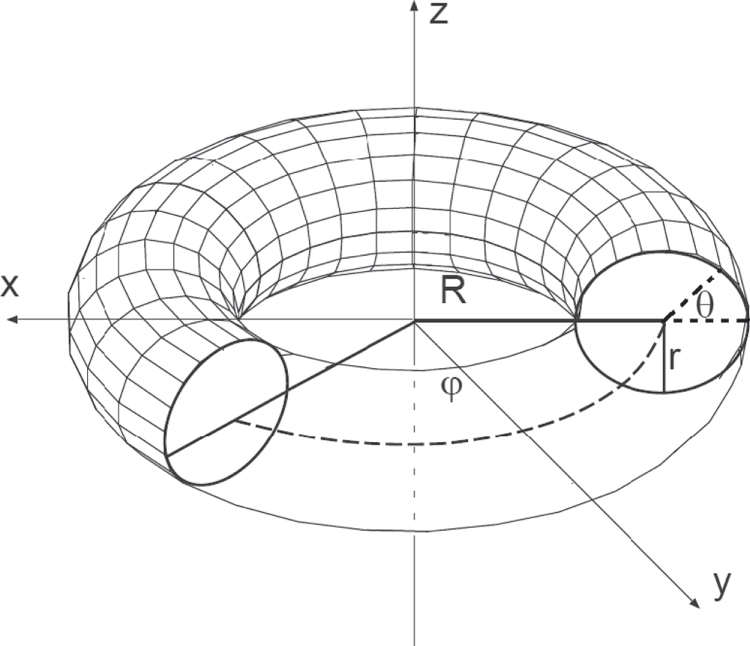
\includegraphics[width=.4\textwidth]{Figures/torus.png}
%        \end{figure}
%        \end{ex}
%        
%        
%        We have given ourselves ways of understanding the scalar functions and curves, but still need to develop a manner to understand vector fields.  We will not only need to understand vector fields in their own right, but we will need them in order to investigate how the scalar fields change from point to point.  Roughly speaking, the ``derivative" of a scalar field will be a vector field.
%        
%        \section{Vector Fields}
%        
%        A vector field is a function that inputs a vector and outputs a vector. Specifically, we can write
%        \[
%        \mathbf{v}(x,y,z)=(f_1(x,y,z),f_2(x,y,z),f_3(x,y,z))=\begin{bmatrix} f_1(x,y,z)\\ f_2(x,y,z) \\ f_3(x,y,z)\end{bmatrix}.
%        \]
%        Notice the differences and similarities between vector fields, scalar fields, and curves.  Just as before, it will be nice to visualize many vector fields in the $xy$-plane to avoid drawing in 3-dimensions. Of course, we can use technology to make nice plots in space.
%        
%        Intuitively, a vector field is an assignment of a vector at each point in space.  To match this intuition we tend to just draw a collection of arrows in space.
%        
%        \begin{ex}{Eastward Wind}{east_wind}
%        Consider the vector field
%        \[
%        \mathbf{v}\colon \R^2 \to \R^2
%        \]
%        given by
%        \[
%        \mathbf{v}(x,y)=(1,0).
%        \]
%        At each point $(x,y)$, we are assigning a vector that points a distance 1 in the $x$-direction. See the following figure.
%        \begin{figure}[H]
%            \centering
%            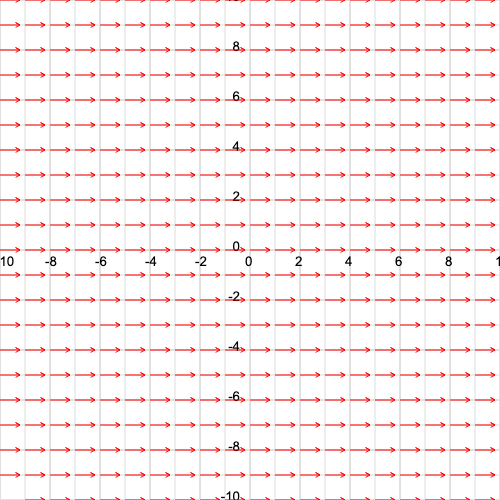
\includegraphics[width=.6\textwidth]{Figures/wind_field.png}
%        \end{figure}
%        \end{ex}
%        
%        \begin{ex}{Line Source}{line_source}
%        Consider the vector field in the plane given by
%        \[
%        \mathbf{v}(x,y)=(x+y,x+y).
%        \]
%        See the following figure.
%        \begin{figure}[H]
%            \centering
%            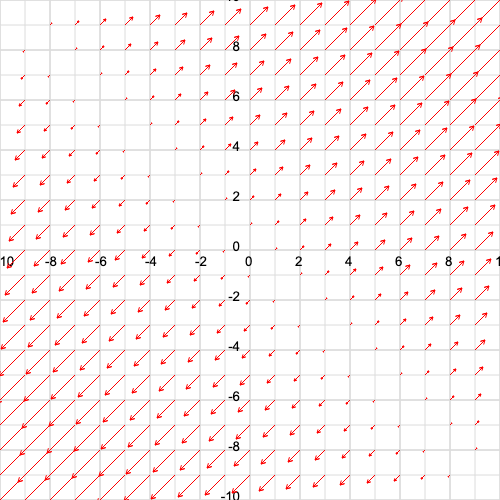
\includegraphics[width=.6\textwidth]{Figures/v_field_1.png}
%        \end{figure}
%        \end{ex}
%        
%        \begin{ex}{Whirlpool}{whirlpool}
%        Consider the vector field in the plane given by
%        \[
%        \mathbf{v}(x,y)=(y,-x).
%        \]
%        See the following figure.
%        \begin{figure}[H]
%            \centering
%            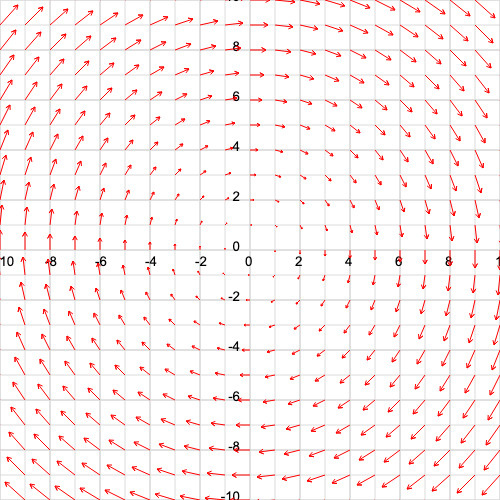
\includegraphics[width=.6\textwidth]{Figures/v_field_3.png}
%        \end{figure}
%        \end{ex}
%        
